
\documentclass[12pt]{article}

% Layout.
\usepackage[top=1in, bottom=0.75in, left=1in, right=1in, headheight=1in, headsep=6pt]{geometry}

% Fonts.
\usepackage{mathptmx}
\usepackage[scaled=0.86]{helvet}
\renewcommand{\emph}[1]{\textsf{\textbf{#1}}}

% TiKZ.
\usepackage{tikz, pgfplots}
\usetikzlibrary{calc}
\pgfplotsset{compat = newest}
 
\pgfplotsset{my style/.append style={axis x line=middle, axis y line=
middle, xlabel={$x$}, ylabel={$y$}, axis equal }}

% Misc packages.
\usepackage{amsmath,amssymb,latexsym}
\usepackage{graphicx}
\usepackage{array}
\usepackage{xcolor}
\usepackage{multicol}

% Commands to set various header/footer components.
\makeatletter
\def\doctitle#1{\gdef\@doctitle{#1}}
\doctitle{Use {\tt\textbackslash doctitle\{MY LABEL\}}.}
\def\docdate#1{\gdef\@docdate{#1}}
\docdate{Use {\tt\textbackslash docdate\{MY DATE\}}.}
\def\doccourse#1{\gdef\@doccourse{#1}}
\let\@doccourse\@empty
\def\docscoring#1{\gdef\@docscoring{#1}}
\let\@docscoring\@empty
\def\docversion#1{\gdef\@docversion{#1}}
\let\@docversion\@empty
\makeatother

% Headers and footers layout.
\makeatletter
\usepackage{fancyhdr}
\pagestyle{fancy}
\fancyhf{} % Clears all headers/footers.
\lhead{\baselineskip 30pt
%\emph{\@doctitle\hfill\@docdate}
\emph{\@docdate\hfill\@doctitle}
\ifnum \value{page} > 1\relax\else\\
\emph{Name: \rule{3.5in}{1pt}\hfill \@docscoring}\fi}
\rfoot{\emph{\@docversion}}
\lfoot{\emph{\@doccourse}}
\cfoot{\emph{\thepage}}
\renewcommand{\headrulewidth}{0pt}%
\makeatother

% Paragraph spacing
\parindent 0pt
\parskip 6pt plus 1pt

% A problem is a section-like command. Use \problem{5} to
% start a problem worth 5 points.
\newcounter{probcount}
\newcounter{subprobcount}
\setcounter{probcount}{0}
\newcommand{\problem}[1]{%
\par
\addvspace{4pt}%
\setcounter{subprobcount}{0}%
\stepcounter{probcount}%
\makebox[0pt][r]{\emph{\arabic{probcount}.}\hskip1ex}\emph{[#1 points]}\hskip1ex}
\newcommand{\thesubproblem}{\emph{\alph{subprobcount}.}}

% Subproblems are an enumerate-like environment with a consistent
% numbering scheme. 
% Use \begin{subproblems}\item...\item...\end{subproblems}
\newenvironment{subproblems}{%
\begin{enumerate}%
\setcounter{enumi}{\value{subprobcount}}%
\renewcommand{\theenumi}{\emph{\alph{enumi}}}}%
{\setcounter{subprobcount}{\value{enumi}}\end{enumerate}}

% Blanks for answers in normal and math mode.
\newcommand{\blank}[1]{\rule{#1}{0.75pt}}
\newcommand{\mblank}[1]{\underline{\hspace{#1}}}
\def\emptybox(#1,#2){\framebox{\parbox[c][#2]{#1}{\rule{0pt}{0pt}}}}

% Misc.
\renewcommand{\d}{\displaystyle}
\newcommand{\ds}{\displaystyle}
\def\bc{\begin{center}}
\def\ec{\end{center}}
\def\be{\begin{enumerate}}
\def\ee{\end{enumerate}}


% Document info
\doctitle{Math F251X: Quiz 8}
\docdate{March 26, 2026}
\doccourse{UAF Calculus I}
\docversion{Spring 2026}
\docscoring{\blank{0.8in} / 25}

\begin{document}

\emph{Please circle your instructor's name:}
\hfill James Gossell \hfill Gordon Williams \\

There are 25 points possible on this quiz.
Any outside materials are not allowed.
\emph{For full credit, show all work clearly.}


\problem{12} The following questions concern the function $f(x)=2x^3-x^4.$
\begin{subproblems}
\item Find $f'(x)$ and identify all critical points of $f(x).$\\
\vfill
\item Determine intervals where $f(x)$ is increasing or decreasing.\\
\vfill
\item Identify the location ($x$-values) of any local maxima or minima of $f(x)$  or state that none exist. 
\vspace{.75in}
\item Find $f''(x)$.
\vspace{.5in}
\item Determine intervals where $f(x)$ is concave up and concave down.
\vfill
\item Identify the $x$-values of any inflection points of $f(x)$ or state that none exist.
\vspace{.75in}
\end{subproblems}

\newpage

\problem{8} Evaluate the given limits. Give the most complete answer possible. If the limit is $\infty$ or $-\infty,$ state this. You must justify your answer algebraically. Answers without any work will not receive full credit.
	\begin{subproblems}
	\item $\displaystyle{\lim_{x \to \infty} \dfrac{x^2-2x^4}{10x^4-x}}$
	\vfill
	\vfill
	\item $\displaystyle{\lim_{x \to - \infty} \dfrac{\sqrt{2x^2}}{x-5}}$
	\vfill
	\vfill
	\vfill
	\end{subproblems}

\problem{5} Below is the \emph{graph of the \underline{derivative} of f(x)}. Use this graph to answer the questions $f(x)$.\\
 
 \begin{multicols}{2}
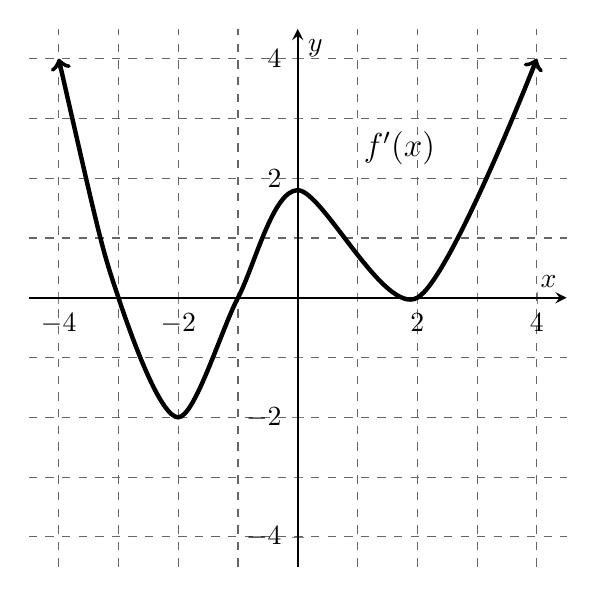
\begin{tikzpicture}
\begin{axis}[scale=1.2, thick, my style, xtick={-4,-2,...,4}, ytick={-4,-2,...,4},
xmin=-4.5, xmax=4.5, ymin=-4.5, ymax=4.5, minor y tick num=1,
        minor x tick num=1, mark size=3.0pt, grid=both, grid style={ thin, black!60, dashed}, axis equal image]
%%Curve
\addplot[ultra thick, smooth,<->] coordinates {(-4,4)(-3,0) (-2,-2) (-1,0)(0,1.8) (2,0)  (4,4)};
\node at (1.7,2.5){\large{$f'(x)$}};
\end{axis}
\end{tikzpicture}
\quad


\quad

\columnbreak

\begin{subproblems}
\item When is $f(x)$ increasing? 
\vfill
\item When is $f(x)$ decreasing?
\vfill
\item Determine where $f(x)$ has a local maximum or a local minimum.
\vfill
\end{subproblems}
\end{multicols}
\vfill
\vfill


\end{document}